\documentclass{standalone}
\usepackage{amsmath,amssymb,mathtools}
\usepackage{tikz}
\usepackage{pgfplots}
\usepackage{pgf}
\begin{document}
	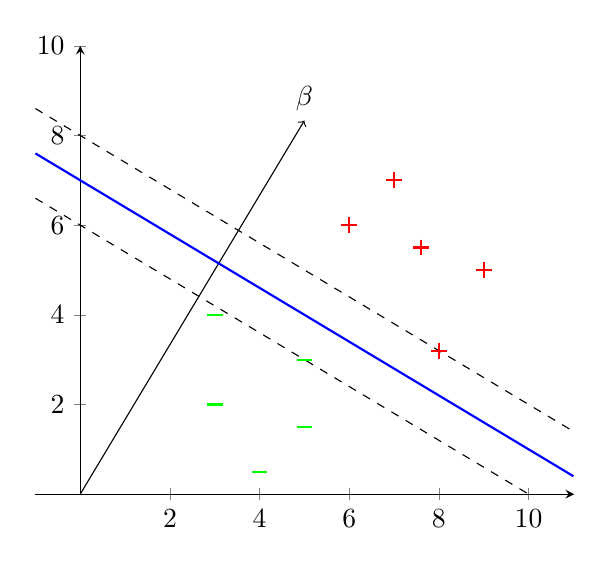
\begin{tikzpicture}
		\begin{axis}[
			xmin=0,
			xmax=10,
			ymin=0,
			ymax=10,
			axis equal,
			axis x line=center,
			axis y line=center
			]
			%\addplot[no markers, domain=-1:11]{(5/3)*x};
			
			\draw[->] (axis cs:0,0)--(axis cs:5,8.333) node[above,pos=1]{$\beta$};
			\addplot[only marks, mark=-,draw=green,mark size=0.1cm,thick]coordinates {(5,3)};
			\addplot[only marks, mark=+,draw=red,mark size=0.1cm,thick]coordinates {(8,3.2)};
			\addplot[only marks, mark=-,draw=green,mark size=0.1cm,thick]coordinates {(3,4)};
			\addplot[only marks, mark=+,draw=red,mark size=0.1cm,thick]coordinates {(7,7)};
			\addplot[only marks, mark=-,draw=green,mark size=0.1cm,thick]coordinates {(5,3)};
			\addplot[only marks, mark=+,draw=red,mark size=0.1cm,thick]coordinates {(8,3.2)};
			\addplot[only marks, mark=-,draw=green,mark size=0.1cm,thick]coordinates {(3,2)};
			\addplot[only marks, mark=+,draw=red,mark size=0.1cm,thick]coordinates {(6,6)};
			\addplot[only marks, mark=-,draw=green,mark size=0.1cm,thick]coordinates {(5,1.5)};
			\addplot[only marks, mark=+,draw=red,mark size=0.1cm,thick]coordinates {(9,5)};
			\addplot[only marks, mark=-,draw=green,mark size=0.1cm,thick]coordinates {(4,0.5)};
			\addplot[only marks, mark=+,draw=red,mark size=0.1cm,thick]coordinates {(7.6,5.5)};
			\addplot[no markers,domain=-1:11,thick,blue]{-0.6*x+7};
			\addplot[no markers, domain=-1:11,dashed]{-0.6*x+8};
			\addplot[no markers, domain=-1:11,dashed]{-0.6*x+6};
		\end{axis}
	\end{tikzpicture}
\end{document}